\documentclass[a4paper]{article}
\usepackage[a4paper,top=2cm,bottom=2.5cm,left=1.5cm,right=1.5cm,marginparwidth=1.75cm]{geometry}
%% Language and font encodings
\usepackage[english]{babel}
\usepackage[utf8x]{inputenc}
\usepackage{listings}

%% Sets page size and margins

\usepackage{float}
%% Useful packages
\usepackage{amsmath}
\usepackage[colorinlistoftodos]{todonotes}
\usepackage[colorlinks=true, allcolors=blue]{hyperref}
\usepackage{listings}
\usepackage{url}
\usepackage{graphicx}
\graphicspath{ {./images/} }
% \DeclareGraphicsExtensions{.pdf,.jpg,.png}

%% defined colors
\definecolor{Blue}{rgb}{0,0,0.5}
\definecolor{Green}{rgb}{0,0.75,0.0}
\definecolor{LightGray}{rgb}{0.6,0.6,0.6}
\definecolor{DarkGray}{rgb}{0.3,0.3,0.3}

\title{Assignment 0: IDS latex template}
\author{
Name1 (s1234567) \\ 
Name2 (s7654321) \\ 
 \\ \textbf{Group} 1234}
\date{\today}


\begin{document}
\maketitle

\abstract{This is the template for writing reports for the weekly assignments. The page 5 pages. You are expected not to change the font size or style or margin width. As in certain conference 
submissions, if the template of your submission deviates significantly from this, your submission might incur negative points. So please follow this template and read the instructions.}
\section*{Introduction}
This template was made for the course introduction to data science \cite{IDS2017}. 
In this section we explain some of the conventions which should be followed for answering theory questions, and how you should organize the report when explaining the experimental part of the 
assignment. Here are some general rules of the report who have to hand in:
\begin{itemize}
 \item You are expected to \textbf{read and follow} instructions via Nestor and Github. Adhere to the rules and conventions of this report template.
 \item The answers to the assignment questions should have number codes as the questions being answered. Students are requested not to change the number codes. For example, if one is writing the 
answer of question 2.1 sub part (a), the answer should have the tag 2.1(a). If the answer to the question 2.1(a) is tagged as II.(i)(a) or 2.1.A or (ii).I.(a) or anything which is different 
from the convention followed in numbering the assignment questions, the answers might be missed and not graded.
\item Do not exceed the page number limit of 5pages , single column.
\item Do not change the font size and page font.
\item Do not change the page margins.
\item Provide snippets of codes in the main report only when \textbf{explicitly} asked for it. Else provide code in Appendices only if you really want to share. 
\item We ask for the codes to be submitted separately anyway. We will run these codes and only if they produce the same figures as those in your report, will your report be validated.
\end{itemize}
The following part guides you on how you should organize the report when answering the practical parts of the assignment, where you have to perform experiments.
\begin{enumerate}
 \item Start with the correct number and letter tag of the question of the assignment.
 \item Provide a \textbf{Motivation} for the experiments [\textit{Had to do it for IDS assignment} or \textit{because the question asked me/us to do} will not be accepted as motivation]. 
 \item Mention the problem statement, where you point out exactly which sub-sets of the issues associated with the \textit{Motivation} you are trying to investigate, and why.
 \item Give a brief overview of what are the available resources and tools which have have in the past and recent past been applied to find solutions to the problems you are trying to handle. 
 \item Explain how your experiment report is organized, i.e., you mention that:
 \begin{itemize}
  \item the first part is the \textbf{Introduction} to the topic, which contains the motivation, problem statement and literature review briefly.
  \item the second part is the \textbf{Methodology} where you have explained briefly the \textit{n} techniques you have used in the concerned experiment.
  \item the third part is the \textbf{Results} where you have put your figures, tables, graphs, etc. 
  \item the fourth part is \textbf{Discussion} where you have discussed the results.
  \item the report ends with a \textbf{Conlcusion} where you have concluded about your findings 
 \end{itemize}

\end{enumerate}

\section{Methodology}
\begin{enumerate}
 \item Give a brief overview (in 1 or 2 sentences) of how you arranged this section,- \textit{name} the techniques that the reader will read, and what kind of a dataset you got and from where.
 \item in \underline{separate sub-sections} now \textit{describe} :
 \begin{itemize}
  \item the different techniques and their pros and cons wrt the problem you are trying to address using them (\textbf{remember to cite your references});
  \item the dataset (no. of dimensions, types of variables in contains, whether labelled or not, and if yes how many classes are there).
  \item how you cleaned the dataset and the preprocessing technique you used.
  \item your experimental setup (you may also show it as a flowchart or block dia
  \item the evaluation measures you used (accuracy/ precision/ AUC/ etc)
 \end{itemize}

\end{enumerate}


\section{Results}
\begin{itemize}
 \item In this section you should have all the figures and tables.
 \item Please ensure that the report shows your figures and tables exactly where you originally intended it to be. 
 The package called \textit{Float} is quite useful for this purpose. 
 \item Please check that your figures and tables contain \textbf{title, and caption}.
 \item Graphs of any kind should have their axes explicitly defined by you.  Also please mention the unit of measurement and keep the tick values of graphs.
 \item If 2 or more figures are to be compared then please ensure that they are in the \underline{same scale}, for not just the benefit of your TAs and instructors, but
 also your own benefit to visualize and interpret your results better.
 \item If your figure contains colour codes, please use \underline{legends} and \underline{colorbars} to help the reader.
\end{itemize}
\begin{figure}[H]
\centering
   
\includegraphics[width=0.5\textwidth]{workClean.png}
   \caption{This figure lacks the axes tick labels and units of measurement. We kindly request you to provide not just axes labels but also axes measurements and units of measurements.}
   \label{fig:noTicks}
\end{figure}
Humour aside, please also avoid the following.
\begin{figure}[H]
\centering
   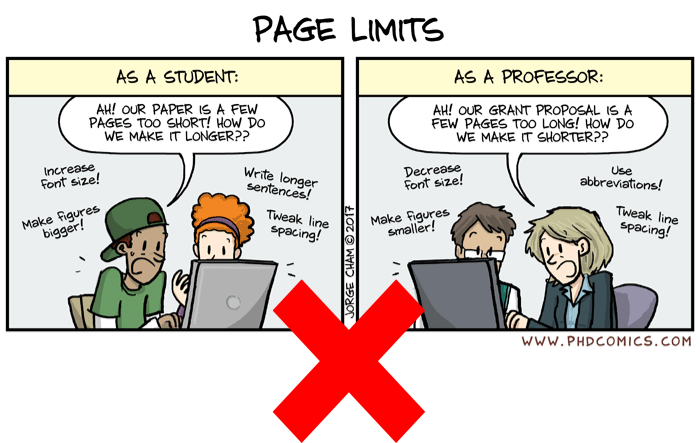
\includegraphics[width=0.5\textwidth]{pageLimit.png}
   \caption{Please try neither. If your figure size is so small that the readability and resolution are compromised, then so shall your grades be. If you have been able to keep your report concise
   and yet been able to describe what you wanted to tell then keep it like that.}
   \label{fig:PageLimit}
\end{figure}
If the titles and axes labels are not readable, they will be considered as absent. 

\begin{figure}[h]
\begin{center}
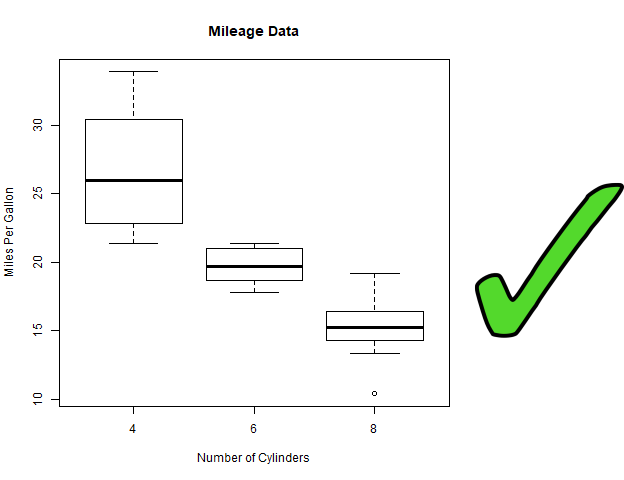
\includegraphics[width=0.5\textwidth]{boxplot}
\caption{Boxplot example from mtcars data.}
\label{fig:rboxplot}
\end{center}
\end{figure}
Figure \ref{fig:rboxplot} was created by the script from tutorialspoint \cite{Rboxplot}. The above is given as an example of an ideal figure. Notice how it contains proper and visible axes, axes labels, 
captions, and title. The figure has good resolution. Produce figures of such quality (with respect to resolution, axes information, label information, units, etc).
\section{Discussion}
Unfortunately due to lack of clairvoyance and omniscience the TAs will not be able to decipher from just your tables and figures what you are trying to suggest, why you did a particular experiment, whether your 
findings are good or bad and if so why. Therefore you are supposed to: 
\begin{enumerate}
 \item provide explanation of the results
 \item guide the TAs and instructors by explaining your results here
 \item explain why a plot or figure supports your hypothesis or not
 \item which technique is better based on which figures and tables
\end{enumerate}
\textbf{Please refer to your figures and tables when discussing them.}
\section{Conclusion}
What is the take home message from this experiment you performed? That is, which techniques do you think work better and why. If you had more time which are some things you would have liked to investigate? Did the 
findings from the experiments you performed support your initial hypothesis? If not, what did you learn from this analysis about the data and about the question whose answer you tried to find with this experiment. 

\bibliographystyle{plain}
\bibliography{bibfile}

\end{document}